%!TEX root=../main.tex

\appendix

\section{A Learning-based Approach}
\label{sec:heuristic}
  
A drawback of the MILP approach is that the generated models grow with the 
size of the database and query log.
However, we argue that encoding the data and query log is necessary to generate a sufficient set of constraints to generate a good repair.
In this section, we examine an alternative, simpler, decision tree-based approach called \dt. 
We show that even in a simple case of a single query log and a complete complaint set, they are expected to perform poorly.
We will first describe how to model the decision tree-based repair process, 
present experimental results, and discuss the reasons for the poor accuracy of \dt.

\subsection{Modeling Repairs with Decision Trees}

\ewu{Justify why using decision trees is the right approach as compared to any other learning algorithm.  
Probably because it is an exemplar rule-based learner, and we believe any other rule-based learner will face the same issues that we find here.} \xlw{NOTES: The bad performance we observe in Figure~\ref{f:heuristic} is mainly caused by server data skew since we keep the same query selectivity when increasing number of tuples. As shown in a survey~\cite{galar2012review}, when 
data get super skewed, none of the classification algorithm works. So, we would still observe the same accuracy even with other algorithms. }

\noindent \textbf{\dt Overview:} Rule-based learners are focused on classification, which naturally matches the goal of solving 
errors in the \texttt{WHERE} clause, however they have no means for dealing with \texttt{SET} clauses, which directly modify data values.
Thus, we take a two step approach, where we first use a classification-based rule learner to generate a repair for the \texttt{WHERE} clause, and use the modified query to identify repairs for the \texttt{SET} clause. 

\noindent
\textbf{Repairing the WHERE Clause:}
The \texttt{WHERE} clause of an update query is equivalent to a
rule-based binary classifier that splits tuples into two groups:
(1)~tuples that satisfy the conditions in the \texttt{WHERE} clause
and (2)~tuples that do not. A mistake in a query predicate can then
result in misclassification: some tuples get classified into the wrong
group, which in turn translates to errors in the data. Therefore,
repairing the mistake corresponds to repairing the imprecise
classification. This works as follows: For an incorrect query $q$, let
$D_0$ be the database state before $q$, and $D_1^*$ the \emph{correct}
database state that should result after $q$.
We use each tuple $t \in D_0$ as an element in the input training data
for the classifier where the values (of each attribute) of $t$ define
the feature vector and the label for $t$:
	\[
    label(t)= 
    \begin{cases}
    true ,& D_0.t \neq D_1^*.t\\
    false,              & \text{otherwise}
    \end{cases}
\]
We then train a rule-based classifier, 
such as decision trees \cite{quinlan1987} to learn
the correct classification rules rules for the \texttt{WHERE} clause.


\noindent
\textbf{Repairing the SET Clause:}
The \texttt{WHERE} clause repair proposed by the classifier may not completely fix 
the complaints if there was also an error in the \texttt{SET} clause.  In these cases,
we execute a second repair step.
We model the errors as a simple linear system of equations: 
each expression in the \texttt{SET} clause is translated into a
linear equation in the same fashion as described in Section~\ref{sec:sol}.
Directly solving for these variables will generate the desired repair for the \texttt{SET} expression.

\subsection{Experimental Results}

  \begin{figure}[h!]
  \centering
    \begin{subfigure} [t]{.75\columnwidth}
    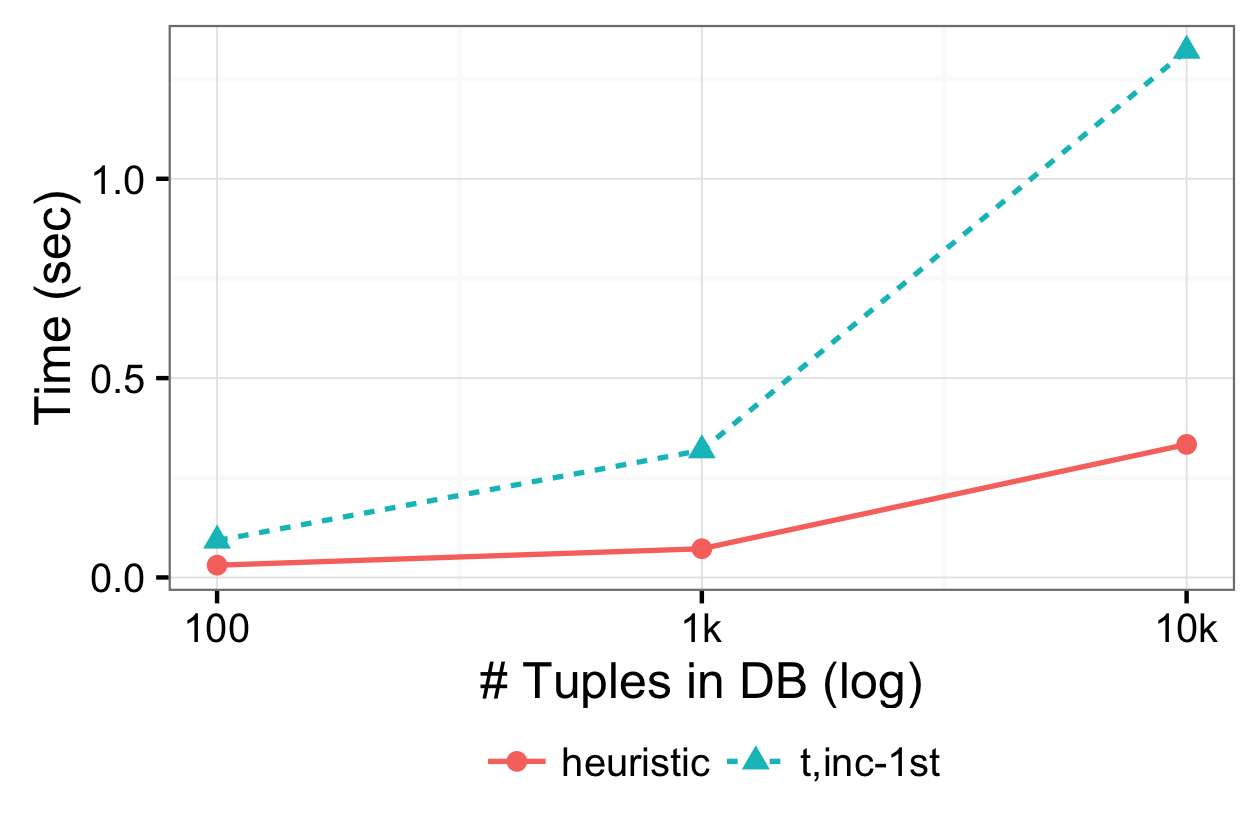
\includegraphics[width = \columnwidth]{figures/heuristictime}
    \caption{Comparison on Performance.}
    \label{f:heuristic_time} 
    \end{subfigure}\\

    \begin{subfigure} [t]{.75\columnwidth}
    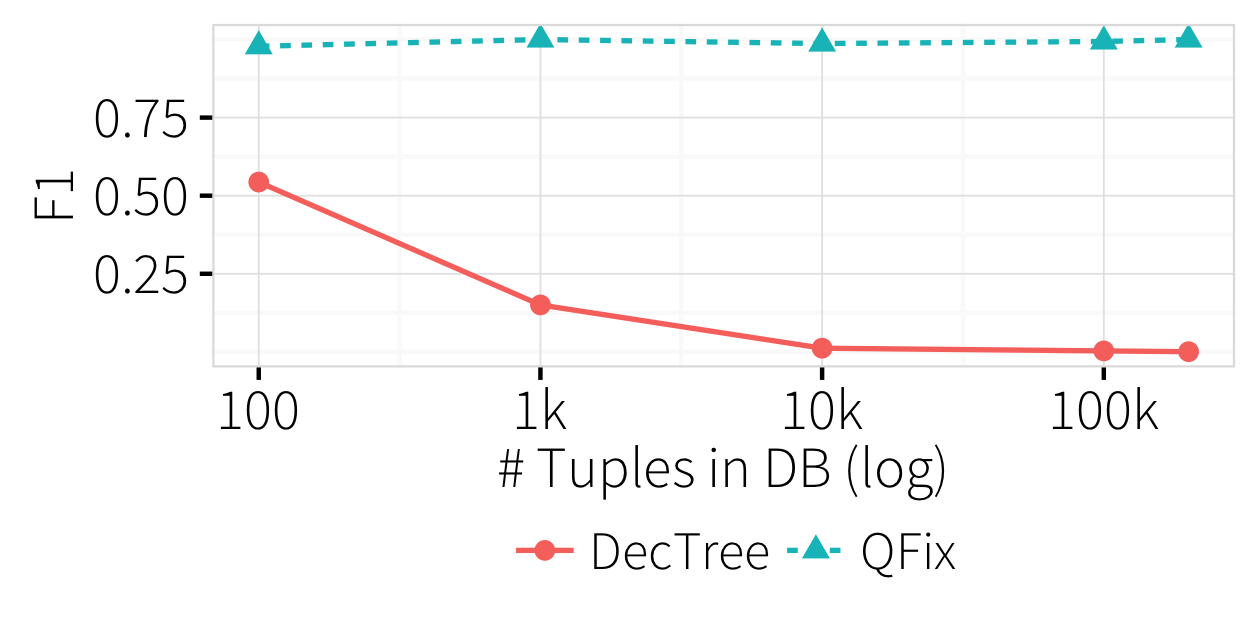
\includegraphics[width = \columnwidth]{figures/heuristicacc}
    \caption{Comparison on Accuracy.}
    \label{f:heuristic_acc} 
    \end{subfigure}
   \caption{\dt compared with \sys}
   \label{f:heuristic}
  \end{figure}


To illustrate these shortcomings, we compare \dt with \sys using a simplified version of the setup from Section~\ref{sec:experiments} that favors \dt.
We restrict the query log to contain a single query that is corrupted, use a complete complaint set  and vary the database size.
The query follows the template:

{\scriptsize
\begin{verbatim}
   SET Clause:                WHERE Clause:
  Constant: SET (a_i=?), ..   Range: WHERE a_j in [?,?+r] & ..
\end{verbatim}
}

Figure~\ref{f:heuristic} shows that although the performance is better by a constant factor ($\sim 2.5 \times$),
\dt scales in a similar manner as \sys.  In addition, the F1-score is consistently below $0.5$ across all database sizes.
From these empirical results, we find that \dt generates low-quality repairs under the simplest conditions---an approach
that applies \dt one query at a time will have little hope.


There are several reasons why \dt, and any approach that focuses on a single query at a 
time\footnote{Although our incremental approach tries to generate a repair for a single
query at a time, it encodes all subsequent queries in the log.}, will not perform well.

\begin{itemize}[itemsep=1pt, leftmargin=5mm]
    
\item \textbf{Single Query Limitation: }
In principle, one could attempt to apply this technique to the
entire log one-query-at-a-time. However, this is not possible in
practice: to learn a classifier on the \texttt{WHERE} clause of query
$q_i$, one needs to know the correct classification output, which
corresponds to \xlw{the previous and next database states 
$D_{i-1}, D_i^*$ of query $q_i$. Unfortunately, deriving the previous 
database state of a query from the later database state is hard without 
knowing any additional information. Thus, even with a complete complaint
set, which can derive the correct database $D_n^*$, there is no
obvious way to ``rollback'' this state to derive $D_i^*$}.
\ewu{this isn't very clear.  Isn't the core reason that any error at any step in the query log will propogate?  Also we need to correctly derive each query's correct previous database state, which is really hard without knowing anything else} \xlw{NOTES: I think the core reason is still we cannot rollback. Even with a clean query log, if we want to figure out the where clause of a query, it is still impossible without a ``rollback'' function. }

\item \textbf{Different Query Structure: } 
\ewu{Can't we just incorporate a distance measure that takes predicate structure into account as part of the decision tree splitting procedure?} \xlw{NOTES: By doing do, we actually modify the objective function of decision tree. This may help improving \dt's performance, but it won't provide any guarantee. Also, we discuss \dt's limitation on single query, and that is the major reason why we don't want to further investigate on this direction. }
The classifier may derive a clause that is structurally very
different from the original one (different attributes or number of
conditions). This is problematic in general, as it corresponds to a
larger-scale mistake in the query, which is a less likely scenario.

\item \textbf{High Selectivity, Low Precision: }
Classifiers try to avoid overfitting, which is problematic for
queries with high selectivity (e.g., single-tuple updates), as the
classifier is unlikely to generate any rules. \xlw{In fact, the problem of learning 
from sever imbalance data is still a great challenge for many major classification algorithms~\cite{he2009learning, galar2012review}. Thus we believe even using alternative classification algorithms, the performance wouldn't be improved as much. In addition, a great percentage of real workloads~\cite{oltpbench} mainly composed by point-update queries which would further worsen the behavior of learning-based approaches.  } 
\ewu{this is called severe class imbalance, would be good to reference some literature in this area.  Decision trees have some issues with sparcity and overfitting}

\end{itemize}


% As shown in Figure~\ref{f:heuristic_acc}, the heuristic approach
% is more efficient than \sys, however, its
% F1-scores are constantly below 0.5 across
% different database sizes where as \sys maintain above 0.9 accuracy. \\
% Therefore, while examining one query at a time by  
% superficially appears
% to be a reasonable and efficient alternative, 
% the reality is that one
% has to model all constraints and transformations through the entire
% log history. In addition, even with single query, though more efficient than \sys, 
% the heuristic alternative can hardly achieve near satisfiable accuracy. 
% 
% The approach that we just described is heuristic in nature. It
% is simple and fast, but it can only process a single incorrect query.
% This results in several shortcomings that make it insufficient in
% practice:





\section{MILP Solver Performance}
\label{app:solvtime}

\ewu{Call it "solver performance" instead of solver solving time}

\ewu{reference other constraint performance papers}
In this section, we study factors that influence the MILP solver solving time. In this paper, we
use IBM CPLEX~\cite{cplex2014v12} as a black box to solve the constructed MILP problems. 
We now directly study the solver behavior and the connection between solver performance on \texttt{UPDATE} workloads and numerous
input factors: the number of constraints, undetermined variables, complaints and queries.

\ewu{XL: more detail on how these experiments are run.  See my edits in previous section for example}
  
  \begin{figure*}[t]
  \centering
      \begin{subfigure} [t]{.3\textwidth}
    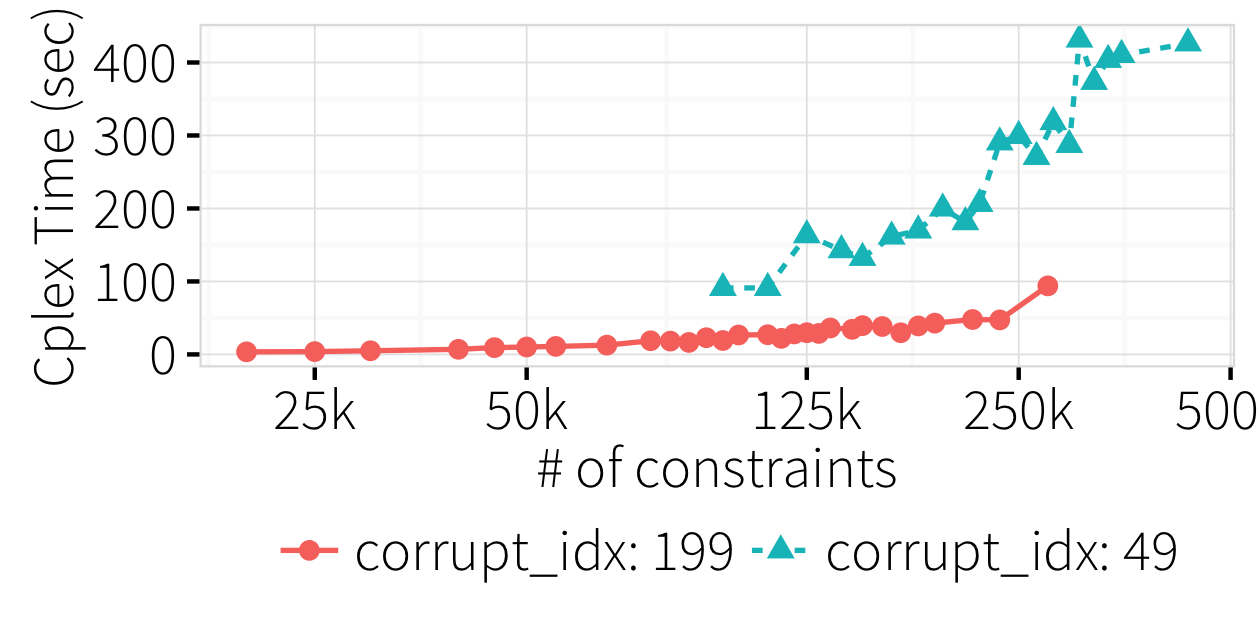
\includegraphics[width = .99\columnwidth]{figures/num_cons_time}
    \vspace*{-.25in}
    \caption{\# of constraints vs. solver solving time.}
    \vspace*{-.1in}
    \label{f:heuristic_time} 
    \end{subfigure}
    \begin{subfigure} [t]{.3\textwidth}
    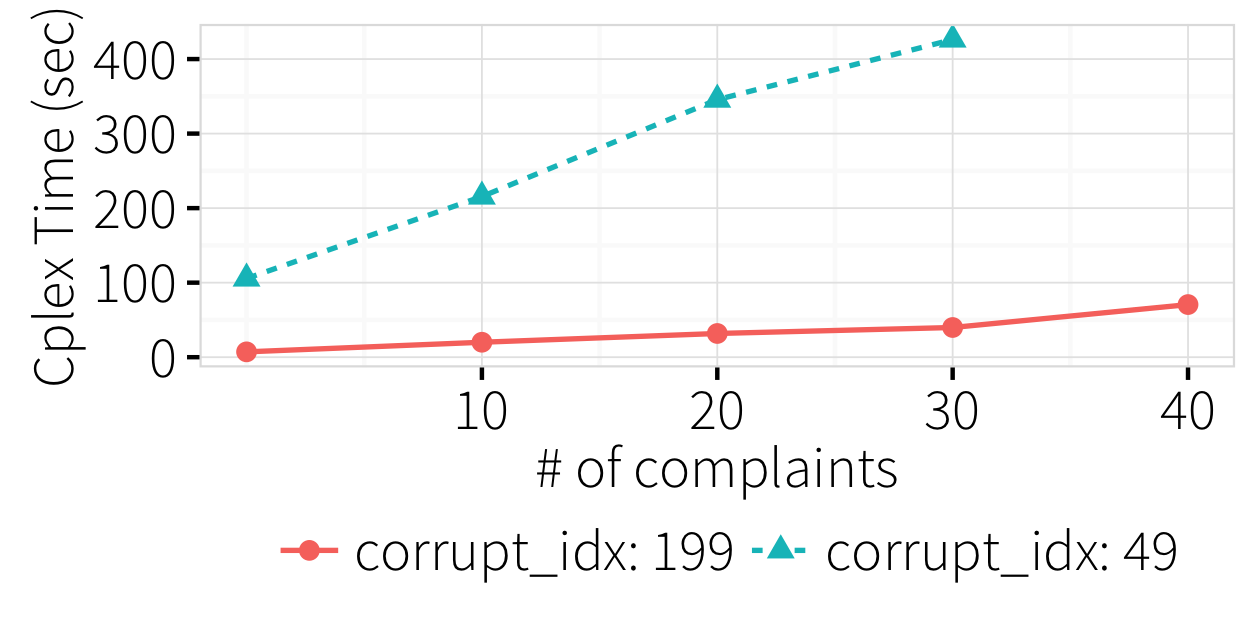
\includegraphics[width = .99\columnwidth]{figures/num_compl_time}
    \vspace*{-.25in}
    \caption{\# of compl. vs. solver solving time.}
    \vspace*{-.1in}
    \label{f:heuristic_acc} 
    \end{subfigure}
    \begin{subfigure} [t]{.3\textwidth}
    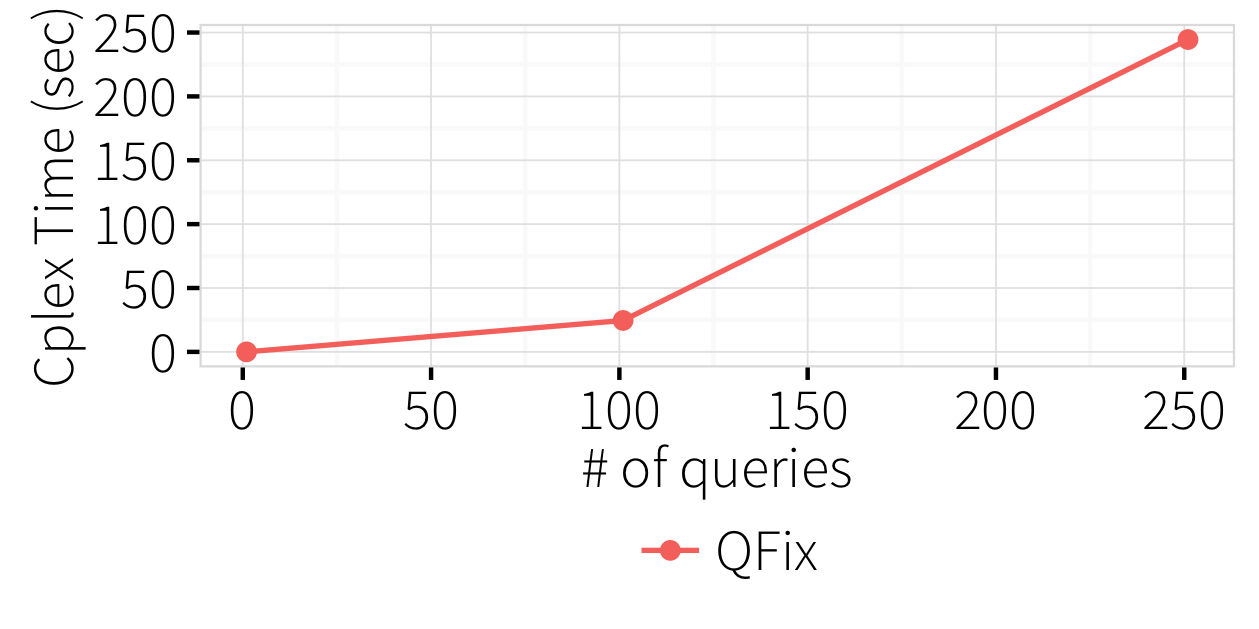
\includegraphics[width = .99\columnwidth]{figures/num_queries_time}
    \vspace*{-.25in}
    \caption{\# of queries vs. solver solving time.}
    \vspace*{-.1in}
    \label{f:heuristic_time} 
    \end{subfigure}
   \caption{Solver solving time grows with all three factors: number of constraints, number of complaints and number of queries. }
   \vspace*{-.1in}
   \label{f:soltime}
  \end{figure*}

  \begin{figure*}[ht]
  \centering
  \begin{subfigure} [t]{.3\textwidth}
    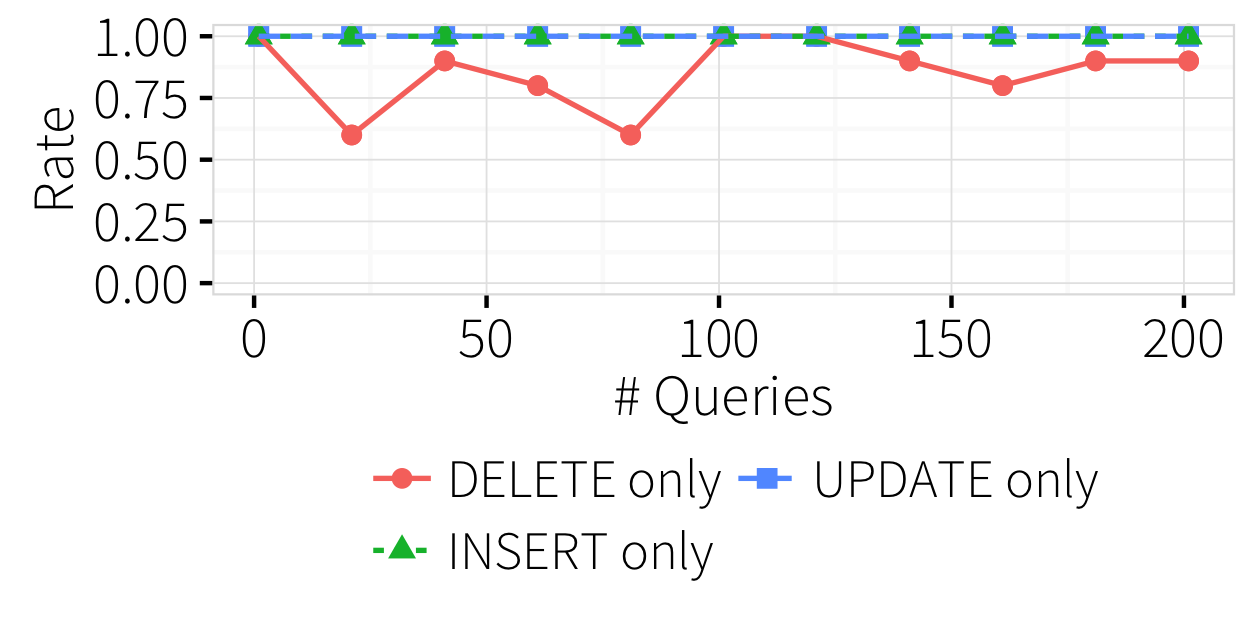
\includegraphics[width = .99\columnwidth]{figures/indelup_acc_idx}
    \vspace*{-.25in}
    \caption{Query types vs. rate of ``true'' fix}
    \vspace*{-.1in}
    \label{f:heuristic_time} 
    \end{subfigure}
    \begin{subfigure} [t]{.3\textwidth}
    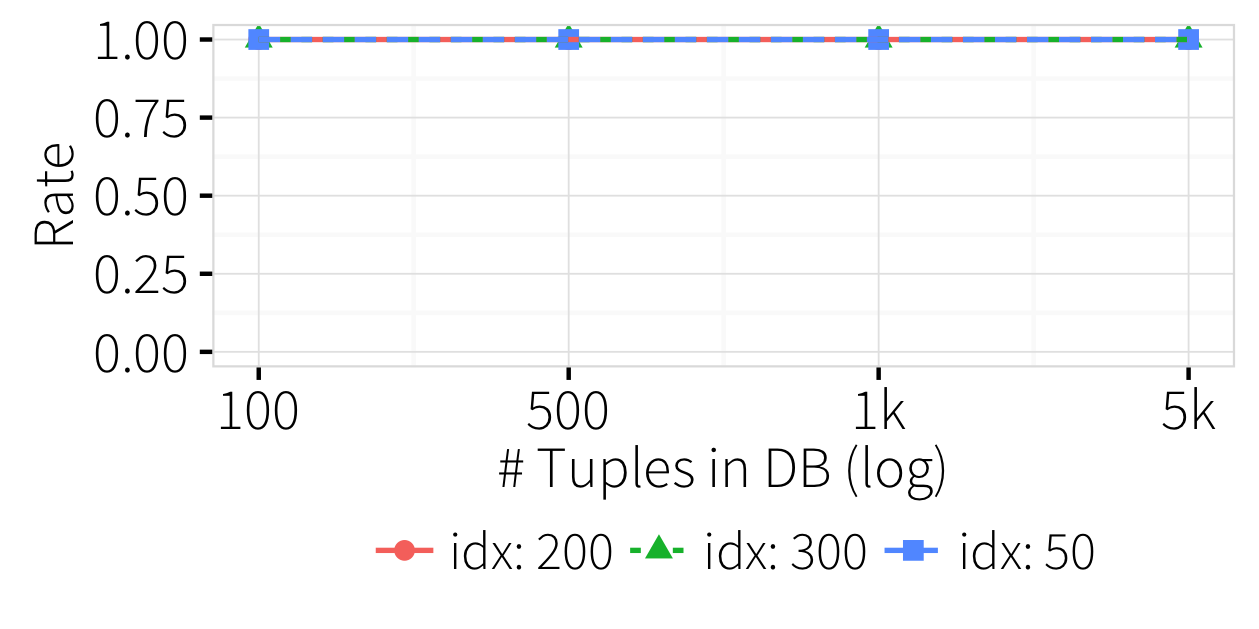
\includegraphics[width = .99\columnwidth]{figures/dbsize_acc_idx}
    \vspace*{-.25in}
    \caption{Database sizes vs. rate of ``true'' fix}
    \vspace*{-.1in}
    \label{f:heuristic_acc} 
    \end{subfigure}
    \begin{subfigure} [t]{.3\textwidth}
    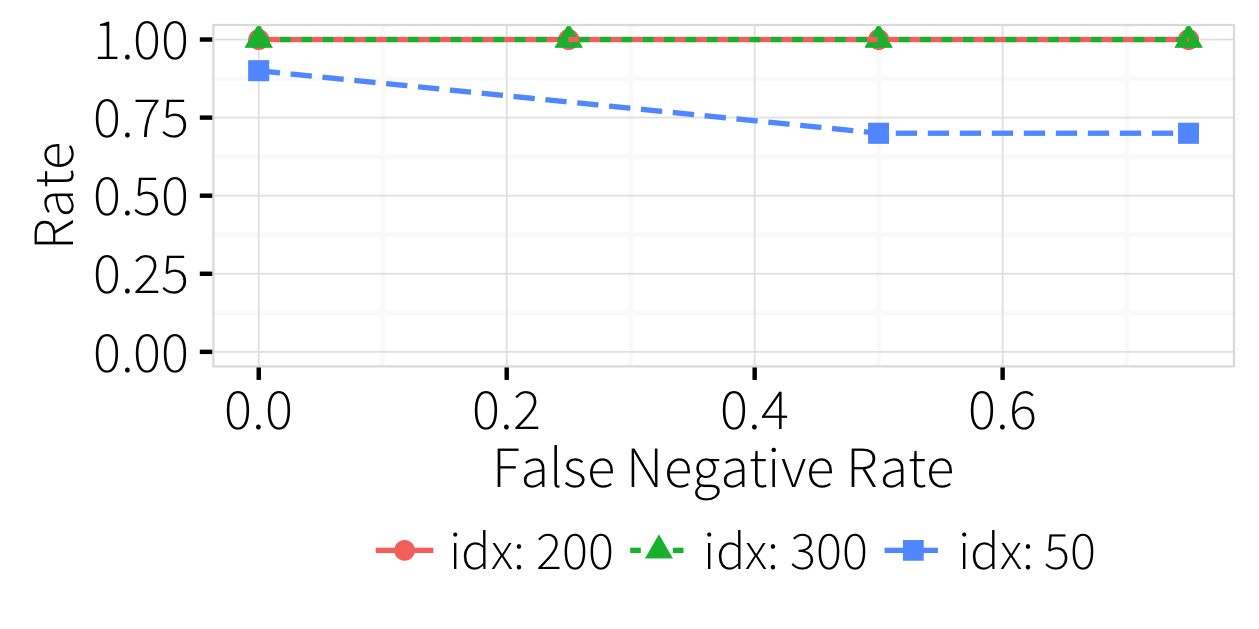
\includegraphics[width = .99\columnwidth]{figures/noise_fn_acc_idx}
    \vspace*{-.25in}
    \caption{False negatives vs. rate of ``true'' fix}
    \vspace*{-.1in}
    \label{f:heuristic_time} 
    \end{subfigure}
   \caption{Rate of ``true'' fix for \sys varies on different types of workloads and false negative rate but remain 
   stable for with increasing number of tuples on \texttt{UPDATE} workload.}
   \vspace*{-.1in}
   \label{fig:truerate}
  \end{figure*}

\smallskip
\emph{Number of Constraints: } We first study the relation between solver solving time and number of constraints and observe that solver solving time is roughly positive proportional, with tiny fluctuation, to the number of constraints in both corrupt indexes (Figure~\ref{f:soltime}(a)). This is expected because increasing the number of constraints by large scale usually accompany with significantly greater amount of variables in the MILP problem, which lead to harder MILP problems by natural. However, MILP problems with slightly larger amount of constraints sometimes could be even easier to solve since the additional constraints help pruning the searching space for similar amount of variables.

\emph{Number of Undetermined Variables: } In our experiments we found that increasing the number of constraints by increasing the database, query log, or complaint set sizes aversely affects the solver performance,
  solver performance has been shown to \emph{improve} as constraints that effectively reduce the problem space are added to the problem.  
  Thus, we now focus on the effects on the number of undetermined variables, which strictly increases the problem space.
  We keep the number of constraints fixed, however increase the number of undetermined variables by \ewu{XL fill in}

\smallskip
\emph{Number of Complaints: } In Figure~\ref{f:soltime}(b) we compare the solver solving 
time with increasing number of complaints. As illustrated in Section~\ref{sec:sol}, 
the size of number of constraints constructed MILP problem grows linearly with the number of complaints. Thus, solver solving time grows with the number of complaints. 
\ewu{Can you plot the number of complaints vs num constraints and num undetermined variables?  That's what really matters right? Same for num queries}


\smallskip
\emph{Number of Queries: }
\ewu{Can cut, since overlaps with experiments in main paper}
We finally compare solver solving time with the number of queries encoded in the MILP problem and find the solver solving time grows exponentially with the number of queries. This again is due to the way we construct the MILP problem: by increasing the number of queries, more variables are introduced, which increase the hardness in solving the problem. 









\section{Repairing the Correct Query}
\label{app:index}

\ewu{
The experimental section (Section~\ref{sec:experiments}) primarily focused on performance and accuracy measures of the repairs, and for space constraints, ignored 
whether the proposed repair was actually the correct query (it is possible we fix an incorrect query in a way that resolves the complaint set).
Although we found \ewu{describe if we picked the right queries in tnhe paper experiments}, we now turn our attention to better understand 
the conditions when we may fix the incorrect query.   We find that under most conditions, we can expect to identify and repair the correct query.
}

\ewu{how many runs are you plotting? May be good to have more than 20 runs, or are you re-using existing experimental runs from the paper?}

\ewu{
To do this we \ewu{Describe experimental setup}.  We use two evaluation metrics to summarize our results over \ewu{X} runs.
The first $p_{correct}$ computes the ratio between the number of runs where \sys correctly repairs the corrupt query and where \sys
repairs the wrong query.  The second metric $topk$ measures the number of repairs that \sys proposes before repairing the true corrupt query.
This metric is useful to quantify the extent that \sys's repairs are false positives (though they may correctly resolve the complaint set).
A smaller $topk$ value suggests that \sys is still effective at providing repair \emph{recommendations} as part of a diagnostic interface.
}


\textbf{Rate of ``true'' fix vs. query types: } In Figure~\ref{fig:truerate}(a), we first evaluate the ``true'' fix rate on three types of workloads: \sys maintains constant and 
\ewu{what does nearly perfect mean?  Quantify how many we missed! e.g., 1 out of 1000 runs}
nearly perfect ``true'' fix rate for \texttt{UPDATE} and \texttt{INSERT} workloads but unstable and much lower rate for \texttt{DELETE} workload. This is expected since more information of the actual incorrectness get maintained through \texttt{UPDATE} queries by the updated tuple values. However, such information get lost and obscured for \texttt{DELETE} queries as those deleted tuples no longer exist in the database. As a result, actual incorrect queries in \texttt{UPDATE} workloads are much easier to identify than those in \texttt{DELETE} workloads. \texttt{INSERT} workloads are easy to fix by natural since each \texttt{INSERT} query only touches one tuple. 
\ewu{talk about negative vs positive examples, why DELETE is harder.  Basically negative examples don't help a learner/solver correctly generalize, so you it is easy to overfit with a delet query that is similar enough.  Positive examples generate actual constraints that help reduce the set of queries that can be modified to repair the complaints. }

\textbf{top k}: TO FILL IN


\textbf{Rate of ``true'' fix vs. database sizes: } We next narrow down to \texttt{UPDATE} workload and evaluate \sys's behavior with increasing amount of tuples in the database. We observe nearly perfect rate on different corrupt indexes in all database sizes (Figure~\ref{fig:truerate}(b)). 

\textbf{Rate of ``true'' fix vs. false negatives: } We finally evaluate \sys on \texttt{UPDATE} workload with increasing false negative rates. Similar to the quality drop in Figure~\ref{f:falsenegative_acc}, we observe the ``true'' fix rate also suffers from less submitted complaints when errors happen early in the query log. However, \sys maintain nearly perfect ``true'' fix rate for more recent errors (corrupt index is 300 and 200). 


\section{Effect of Index of Corrupted Query}
\label{app:qidx}


A key parameter for our experiments is the location of the corrupted query ($idx$).  
This parameter determines the number of queries \sys must consider when searching for a fix,
and affects the size of the complaint set.  
Both of these characteristics directly impact \sys's 
runtime performance. For this reason, it is undesirable to randomly pick and corrupt queries
throughout the query log, as the performance and accuracy results may not be comparable. 
To better understand the relationship between $idx$ and the size of the complaint set, we ran
simulations using a database with $20$ attributes, and a query log of size $1000$ containing
either all $set = const$ or $set = rel$ \texttt{UPDATE} queries.
We varied  $idx$ uniformly throughout the query log, and additionally varied
the skew $s$ and range $r$ parameters to study how they affect the size of the complaint sets.


  \begin{figure}[h]
  \centering
  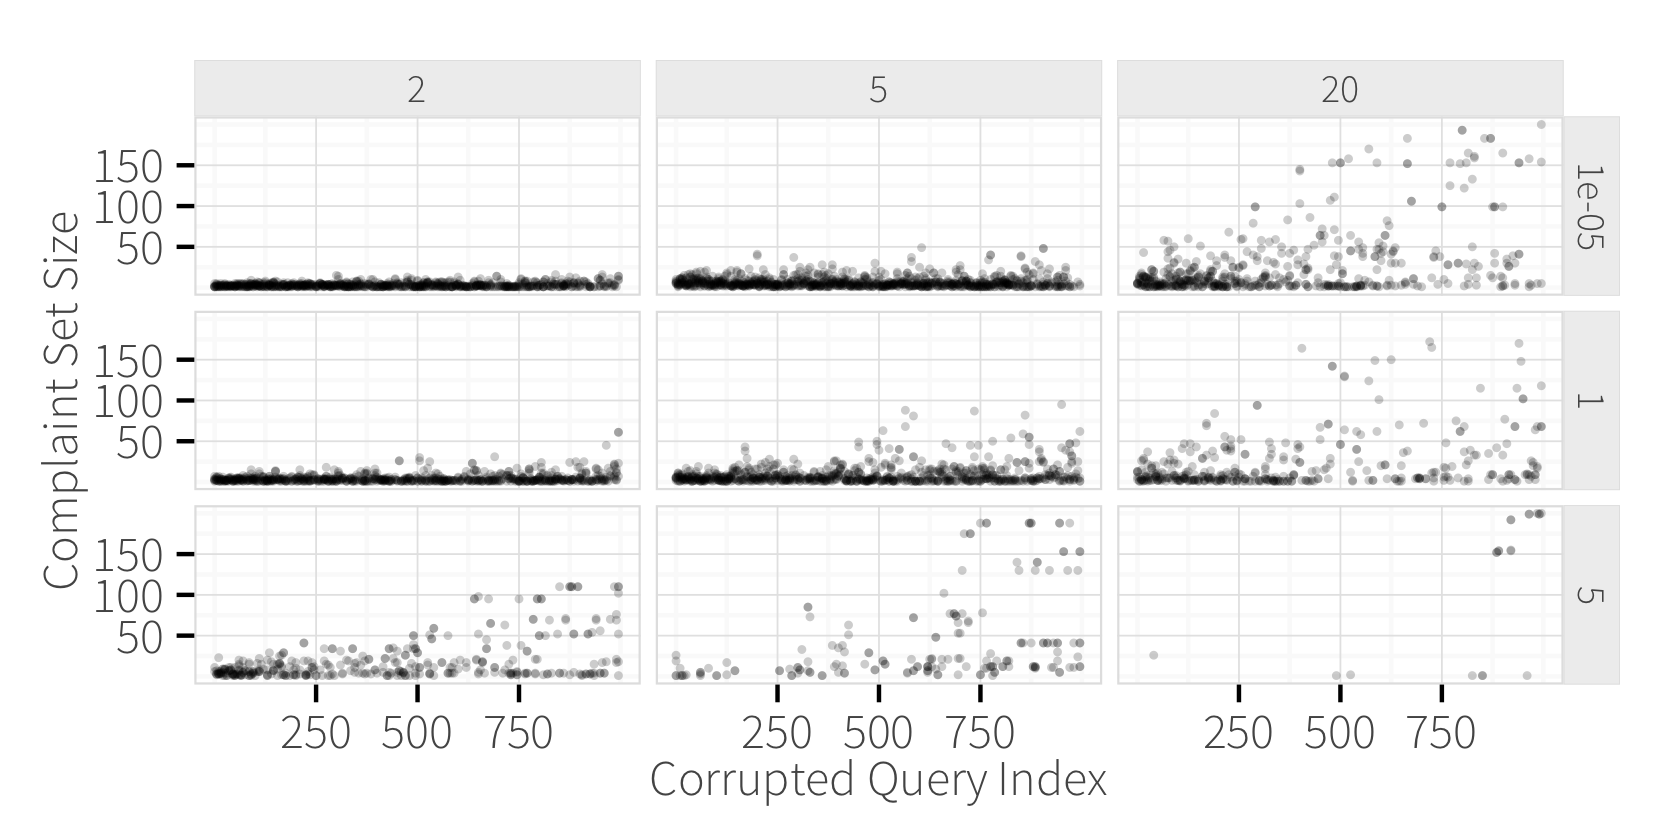
\includegraphics[width = 3.5in]{figures/qidxsimulation/qidx_v_ncomplaints_20attrs_const}
  \caption{Query index vs complaint set size for $set = const$.}
  \label{f:qidx_v_ncomplaints_const} 
  \end{figure}


Figure~\ref{f:qidx_v_ncomplaints_const} plots a representative set of parameters.  We plot one point
for each corrupted query index that results in a complaint set with at least one complaint. 
These results highlight several interesting trends.  When queries do not overlap ($r = 1$, leftmost column),
the size of the complaint sets are relatively small, and their frequency is constant across the possible query indices.
However as the possibility of overlap increases (e.g., $r$ increases), more recent queries are more likely to result in
very large complaint sets (at times the size of the database).   
This effect is a symptom of the fact that queries with large ranges will set groups of tuples to the same value,
and over time, skew the distribution of tuple values to a small number of possible values.
Thus, more recent corruptions that affect a large cluster of similar tuples will result in a large complaint set.
We find that increasing the skew parameter also exacerbates this effect.  
In addition, high skew increases the likelihood that queries will share the same \texttt{WHERE} and \texttt{SET} clause 
attributes as a corrupted query, thus overwriting the error introduced by the corrupted query.  
This is why the frequency of non-empty complaint sets decreases significantly as $s$ increases.


\begin{figure}[h]
\centering
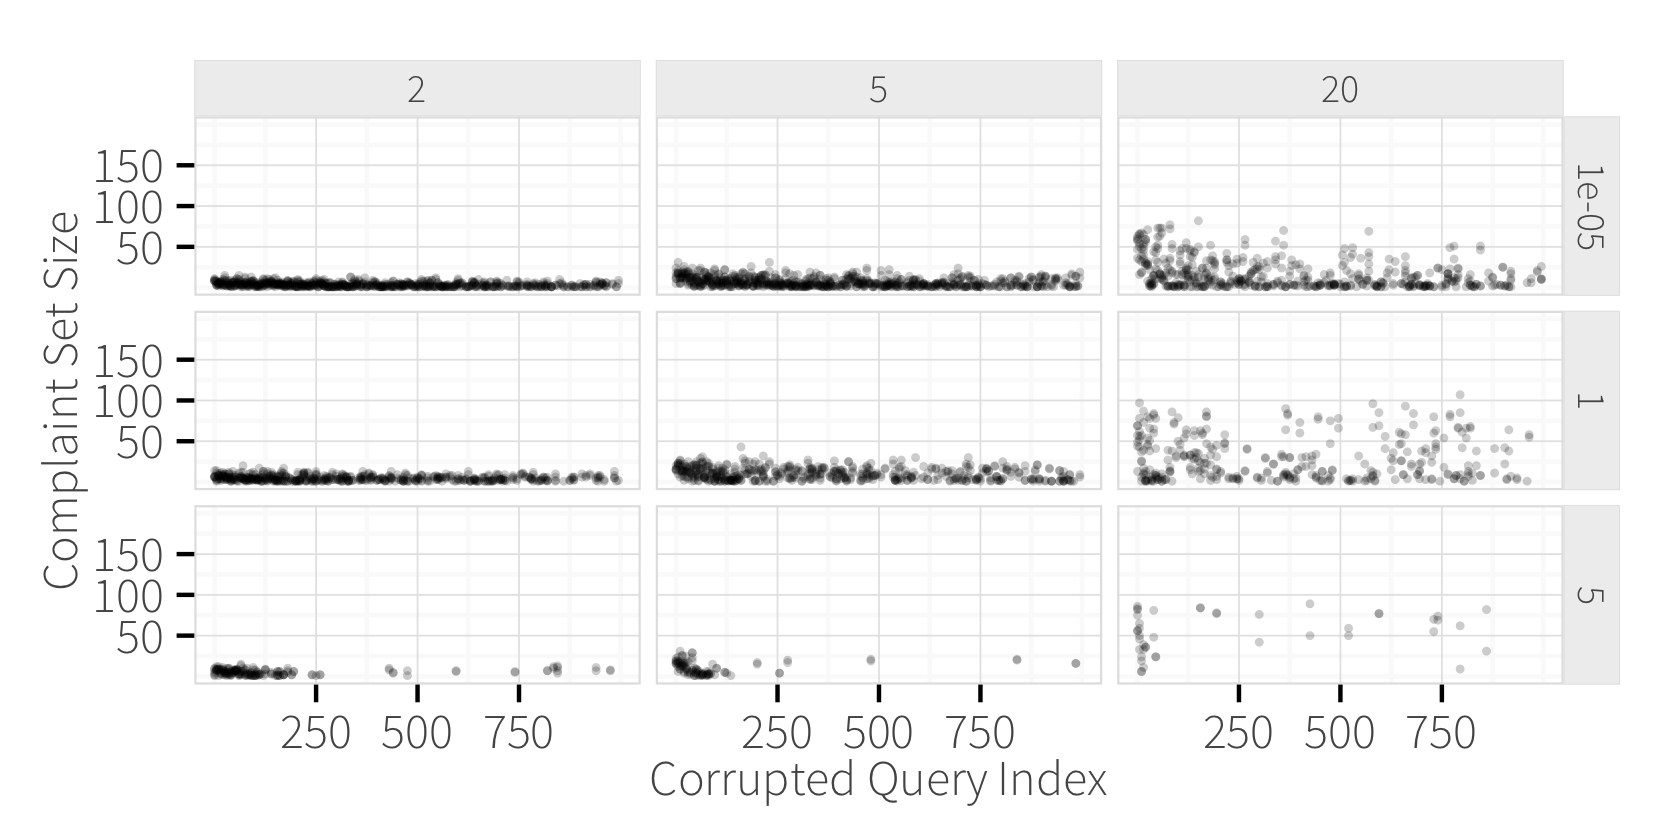
\includegraphics[width = 3.5in]{figures/qidxsimulation/qidx_v_ncomplaints_20attrs_rel}
\caption{Query index vs complaint set size for $set = rel$.}
\label{f:qidx_v_ncomplaints_rel} 
\end{figure}

In contrast to $set=const$ queries, Figure~\ref{f:qidx_v_ncomplaints_rel} executes the 
same experiment using $set=rel$ queries.  In this setting, we find that the trend is
reversed, and older corruptions tend to result in larger complaint sets.  This is because,
subsequent \texttt{UPDATE} queries increment or decrement the attribute value, rather than
overwriting it with a constant value.  The clustering of data values due to query overlap
then increases the number of other tuples affected.


\ewu{summarize findings and implications to experiments here.}
not all corruptions result in complaint sets.
In constant SET clause workloads, larger complaints sets are more likely to
result from more recent corrupted queries -- particularly if the queries are range updates or
the updated attributes are skewed.
For this reason, our experiments corrupt the query log at six positions 
$idx \in \{0, 25, 50, 100, 200, 250\}$ , relative 
to the most recent query (e.g., the most recent query, the $25^th$ most recent query, and so on).

% \begin{figure}[h]
% \centering
% 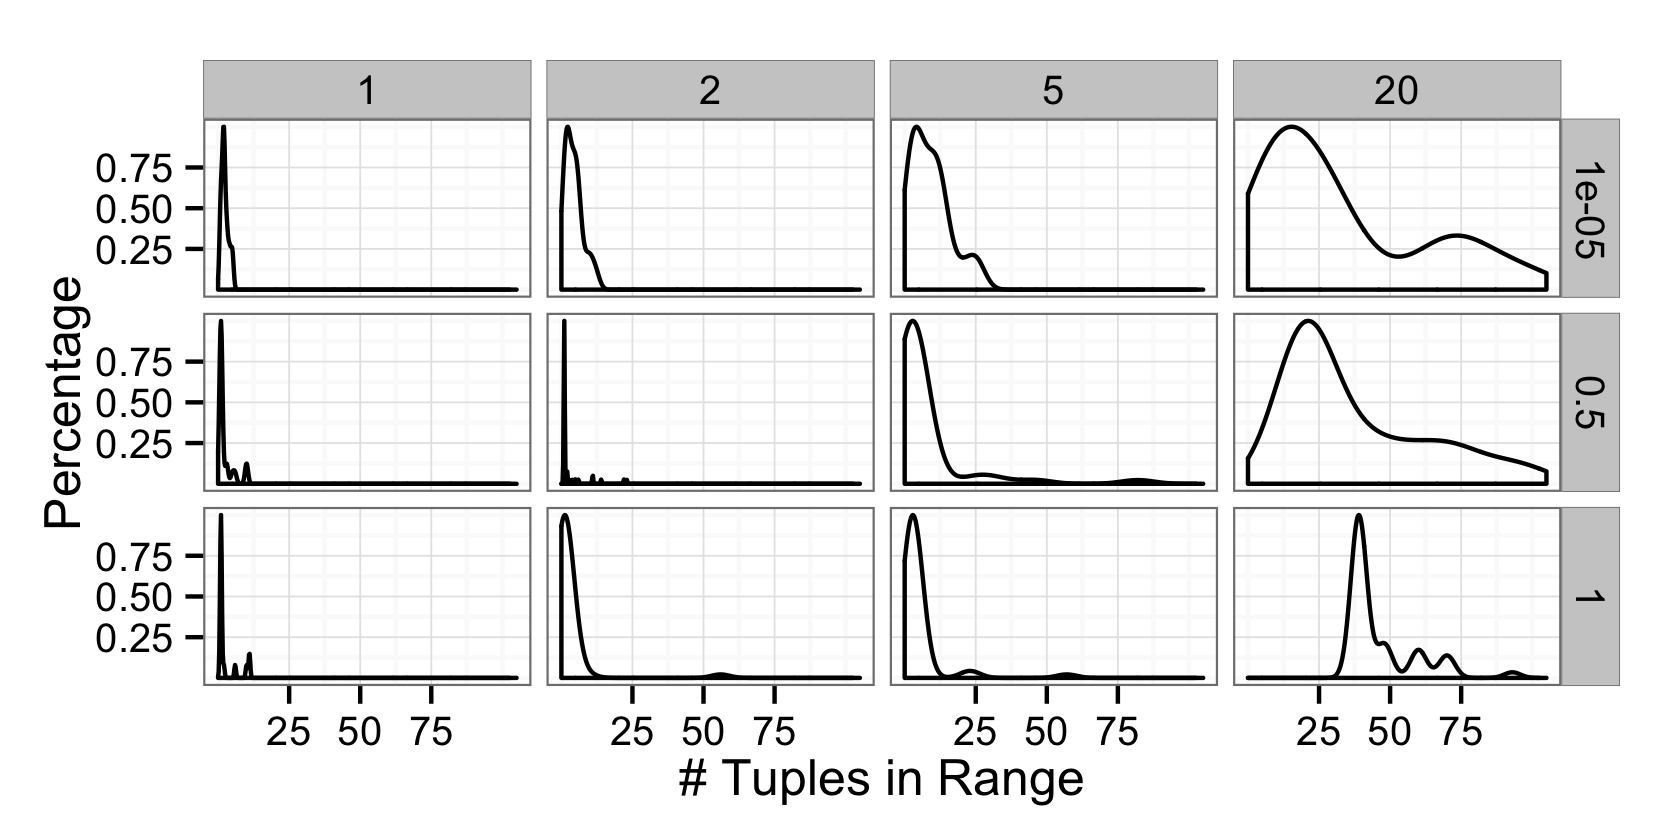
\includegraphics[width = 3.5in]{figures/qidxsimulation/numinrange}
% \caption{.}
% \label{f:numinrange} 
% \end{figure}


As we observed from Figure~\ref{f:multiquery}, \milpall maintains high accuracy when errors
happen more recent, however it does not scale when the error locate further from the most
recent query. \milptuple scales better than \milpall, but ignoring tuples not 
in the complaint set apparently hurts the precision. \milptuplestopearly run times faster
than \milpall and \milptuple, however the aggressive strategy greatly reduce the 
precision. In the end, \milpadvtuple significantly improves the precision with very limited
time cost compare to \milptuple. \\
Based on these observations, we only include the performance of \milpadvtuple and \milpadvall
in the rest of the experiments. 

